\section{Pouzdro}

V~rámci popularizace technologie se~může hodit projektor předvádět na~různých místech. Proto bude potřeba, aby byl projektor přenosný a~při přemisťování se~nerozbil.

Pouzdro je~tedy navrženo tak, aby bylo odolné proti nárazům a~zachovalo všechny součásti v~bezpečí. Každá součástka má své místo, kde je~držena ze~všech stran. Pro výrobu pouzdra by~bylo vhodné využít technologii 3D tisku. Ta~umožňuje tvorbu komplexních geometrických tvarů přímo pro potřeby konkrétního modelu a~zároveň umožňuje snadnou iteraci a~úpravu designu pouzdra při nalezení chyb.

Pouzdro bylo navrženo v programu Autodesk Fusion.

\subsection{Priority designu} \label{sec:krabick-design-priorities}
\subsubsection{Chlazení}
Největší část projektoru je~hliníkový chladič s~větrákem. Už od~začátku práce byl tento chladič vybrán, aby byl připevněn k~řídící desce galvanometrů. Problematika jejího zahřívání je~popsaná v~kapitole~\ref{sec:galvoboard-chips-heating-up}.
Jak bylo popsáno v~této kapitole, na~řídící desce galvanometrů je~připevněna hliníková destička, která chladí čipy. Chladič byl připevněn právě na~ni.

Aktivní chladič\footnote{Chladič s~větrákem, který aktivně vytváří proud vzduchu} se~ale hodí i~pro ostatní součástky. Vzduch, který nasaje je~totiž distribuován celou vnitřní konstrukcí projektoru a~chladí tak všechny vnitřní součástky. Tomuto proudění byla věnována zvláštní pozornost při designu konstrukce pouzdra.

\subsubsection{Přístup k~portům Raspberry Pi}
Aby bylo možné je používat, je potřeba zajistit jednoduchý přístup k portům Raspberry Pi. Dále je potřeba od nich odlišit nabíjecí port.

\subsubsection{Modularita, jednoduchá konstrukce}
Pouzdro bylo designováno také aby bylo modulární. Aby bylo možné při prototypování vyměnit pouze jednu součástku, která nesedí místo tisknutí celého pouzdra od~začátku. S~modularitou bylo zároveň dosaženo jednoduché konstrukce, v~jakékoliv části stavby je~možné dočasně odstranit díly, aby bylo možné upravit připevnění vnitřní elektroniky.

\subsection{Konstrukce}
Pouzdro se~skládá ze~čtyř vertikálních stěn s~otvory, do~kterých zapadají horizontální desky. Horizontální desky v~sobě mají vždy z~vrchní strany vyhloubené prohlubně, do~kterých pasují elektronické součástky, které na~nich leží. Díky tomu se~elektronické součástky při pohybu projektoru volně nepohybují ve~vnitřních prostorách.

\begin{figure}[htb]
  \centering
  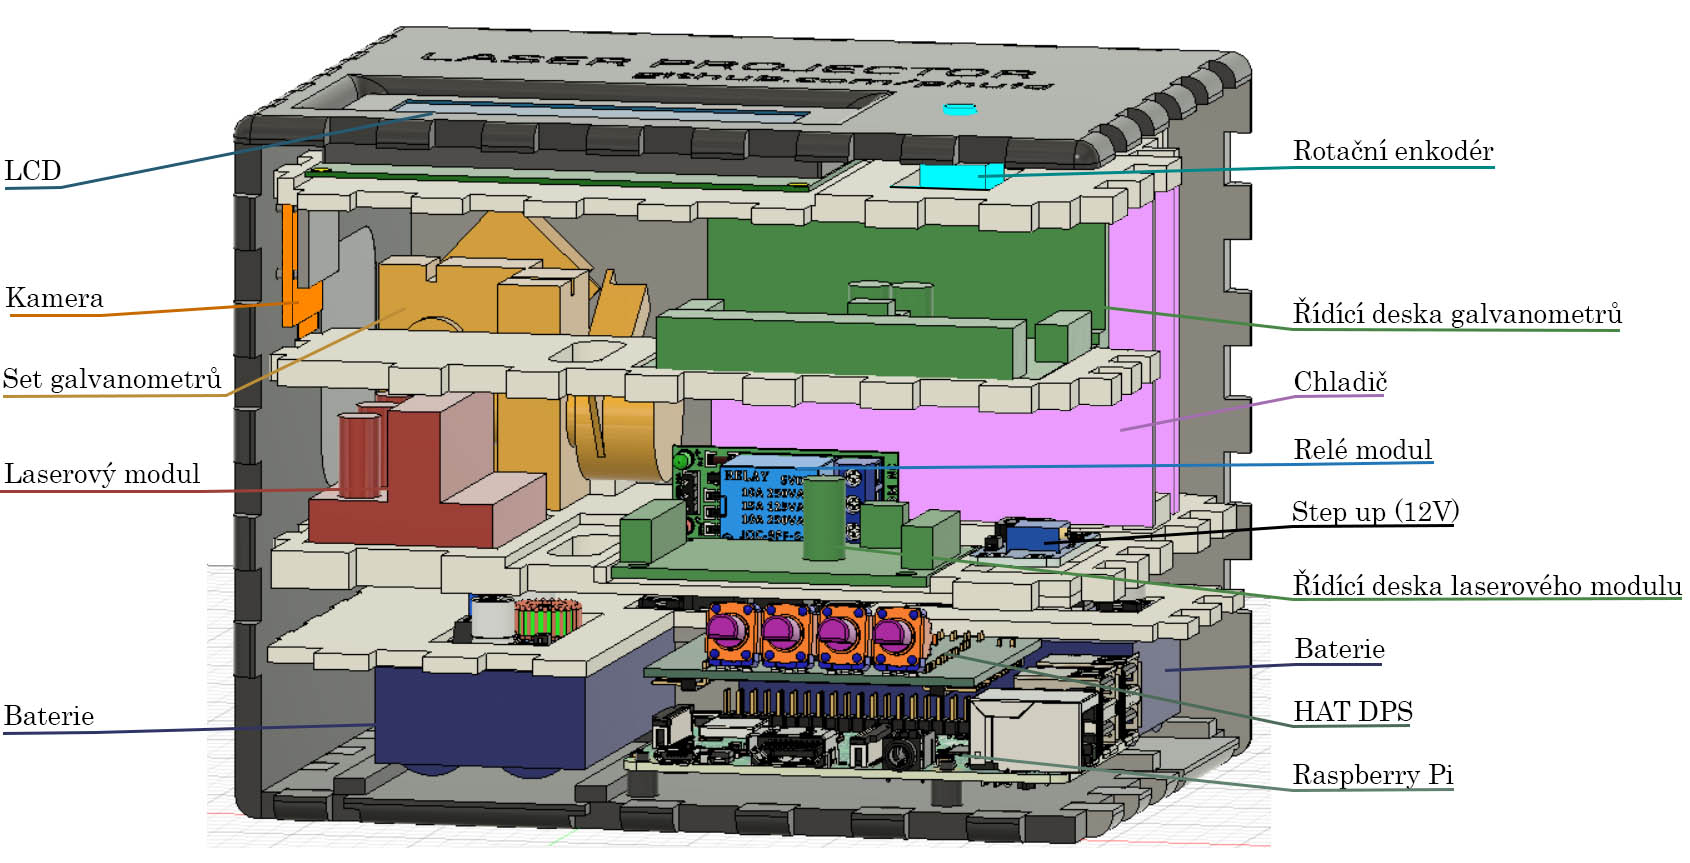
\includegraphics[width=1\textwidth]{img/case-sideview.jpg}
  \caption{\label{fig:case-sideview} Pohled do~projektoru s odstraněnou přední stěnou v programu Autodesk Fusion}
\end{figure}

Tyto prohlubně jsou hlavní důvod, proč byl k~výrobě dílů využit 3D tisk místo například laserového řezání.

Elektronika je~v prohlubních často držena i lepidlem z~tavné pistole.
To bylo přidáno s původním cílem upevnit k elektronice kabely z~ní vedoucí i za~izolaci. Kdyby kabely držely jen za~vodičové drátky k elektronice připájené, drátky by~se v průběhu času kvůli vibracím při přenášení polámaly.

Jak je~vidět na~obrázku~\ref{fig:case-sideview}, pouzdro je~rozděleno do~pěti pater. Jednotlivá patra nezabírají celou plochu horizontální plochu projektoru. Často spojují pouze tři ze~čtyř stěn, nebo jsou v nich otvory, kterými může proudit vzduch. V prvním patře se~nachází baterie (zvýrazněny modře), destička s BMS obvodem a~v neposlední řadě Raspberry Pi. Na~něm je~připevněná HAT deska plošných spojů, která zasahuje do~druhého patra. Druhé patro je~vidět na~obrázku~\ref{fig:hw_layer0} a~nachází se~v něm obvod nabíjení baterie (PD trigger deska, step up~měnič a~nabíječka Li-ion článků).
Dále se~v něm nachází step down měnič napájející Raspberry Pi~a~step up~měnič napájející galvanometry.

\begin{figure}[htb]
  \centering
  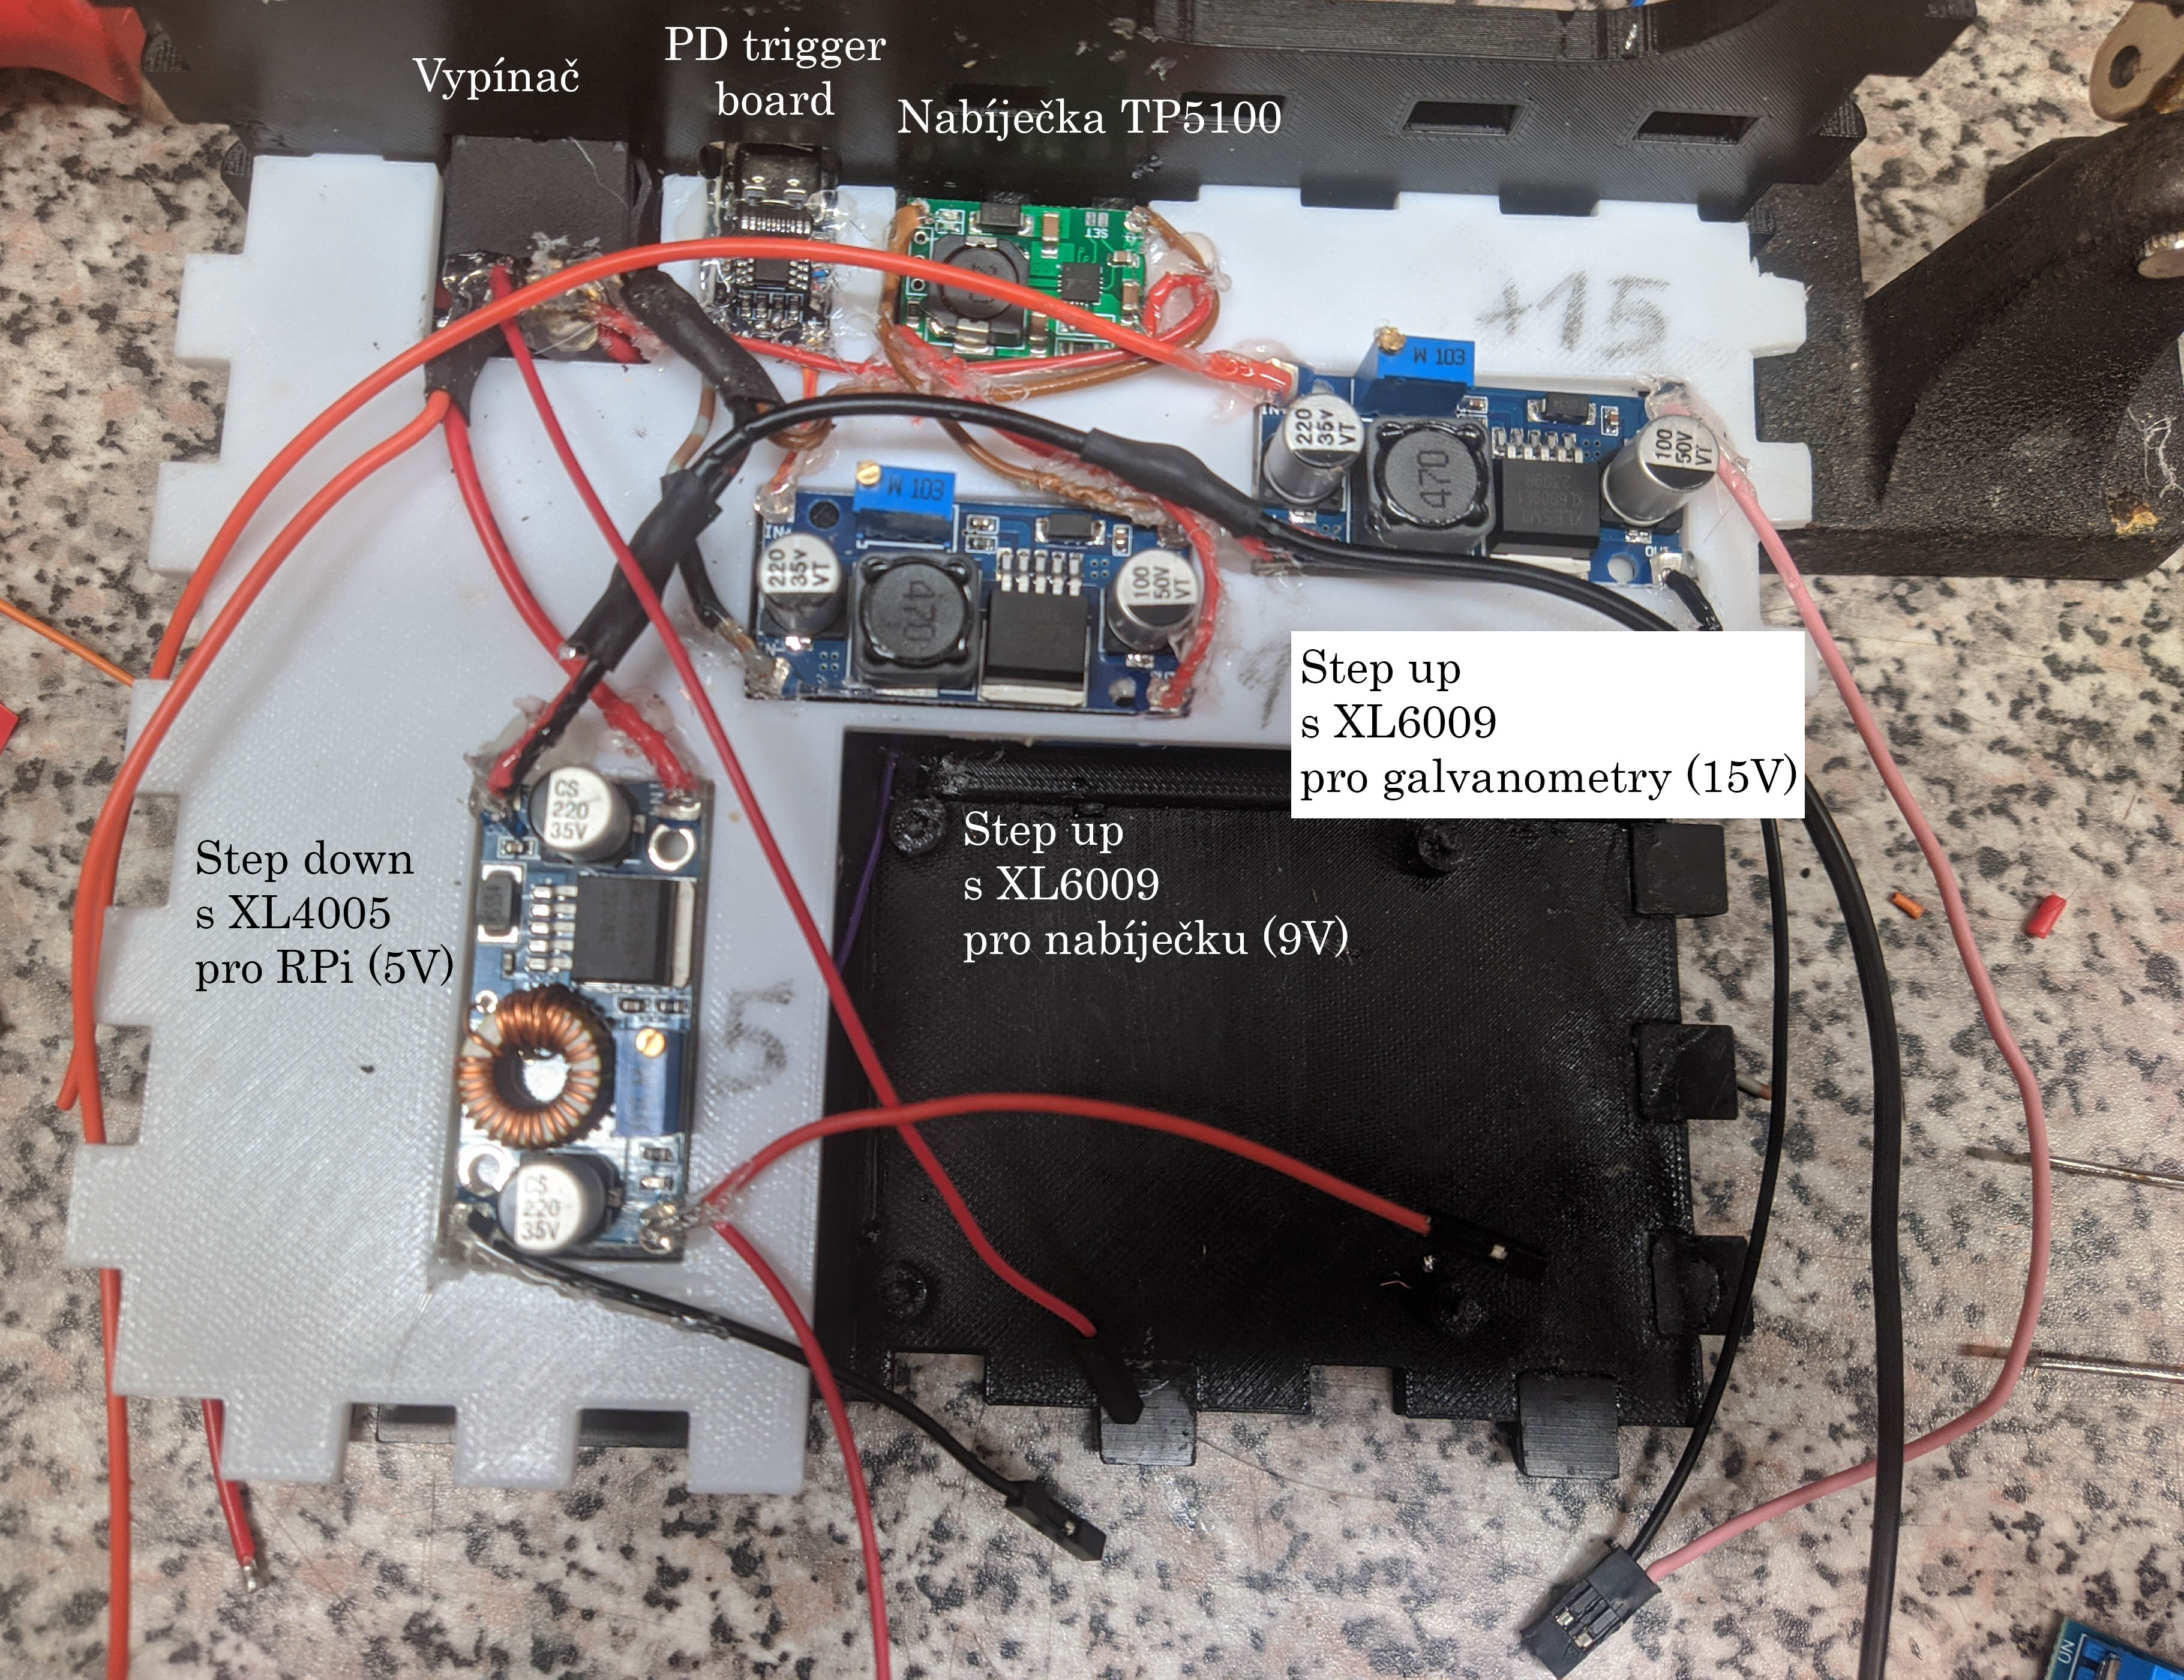
\includegraphics[width=0.8\textwidth]{img/hw_layer0.jpg}
  \caption{\label{fig:hw_layer0} Kompletně nainstalované druhé patro (Na obrázku je~modul TP5100 zapojen s opačnou polaritou, ve~výrobku byla chyba opravena, ale tato fotka je~stále nejlepší ilustrace.)}
\end{figure}

Ve třetím patře je~upeněn chladič, foukající na~nabíjecí obvod a~step up~měniče pod ním, set galvanometrů (zvýrazněn žlutě), laserový modul (zvýrazněn červeně) a~jeho řídící deska (zvýrazněna zeleně), step up~měnič pro laser a~relé modul.  
Galvanometry zasahují až do~čtvrtého patra, kde je~upevněna jejich řídící deska. Ta je mimo jiné připevněna na chladič párem šroubků viditelných na obrázku~\ref{fig:hw_galvoboard} ze strany \pageref{fig:hw_galvoboard}, mezi desku a chladič byla aplikována teplovodivá pasta. V prostorách čtvrtého patra je~také na~stěnu upevněna kamera.
V pátém patře se~nachází LCD a~rotační enkodér.

V horizontálních deskách oddělujících patra od~sebe jsou otvory pro vzduch, jak zmíněno v sekci~\ref{sec:krabick-design-priorities}, také na~přední stěně pouzdra jsou otvory pro vyfukování vzduchu. Na~přední stěně je~také otvor pro přístup k potenciometrům na~HAT DPS a~otvor pro přístup k portům Raspberry Pi, ten je~i na~pravé boční stěně. Na~zadní stěně je~otvor pro nasávání vzduchu větrákem, vypínač, a~otvory pro USB-C port PD trigger desky a~statusové diody nabíječky TP5100. Na~levé boční stěně jsou pak otvory pro kameru a~laserový výstup galvanometrů. Ve~dně jsou otvory pro výmněnu baterií a~ve~stropní stěně jsou otvory pro LCD a~rotační enkodér.

\begin{figure}[htb]
  \centering
  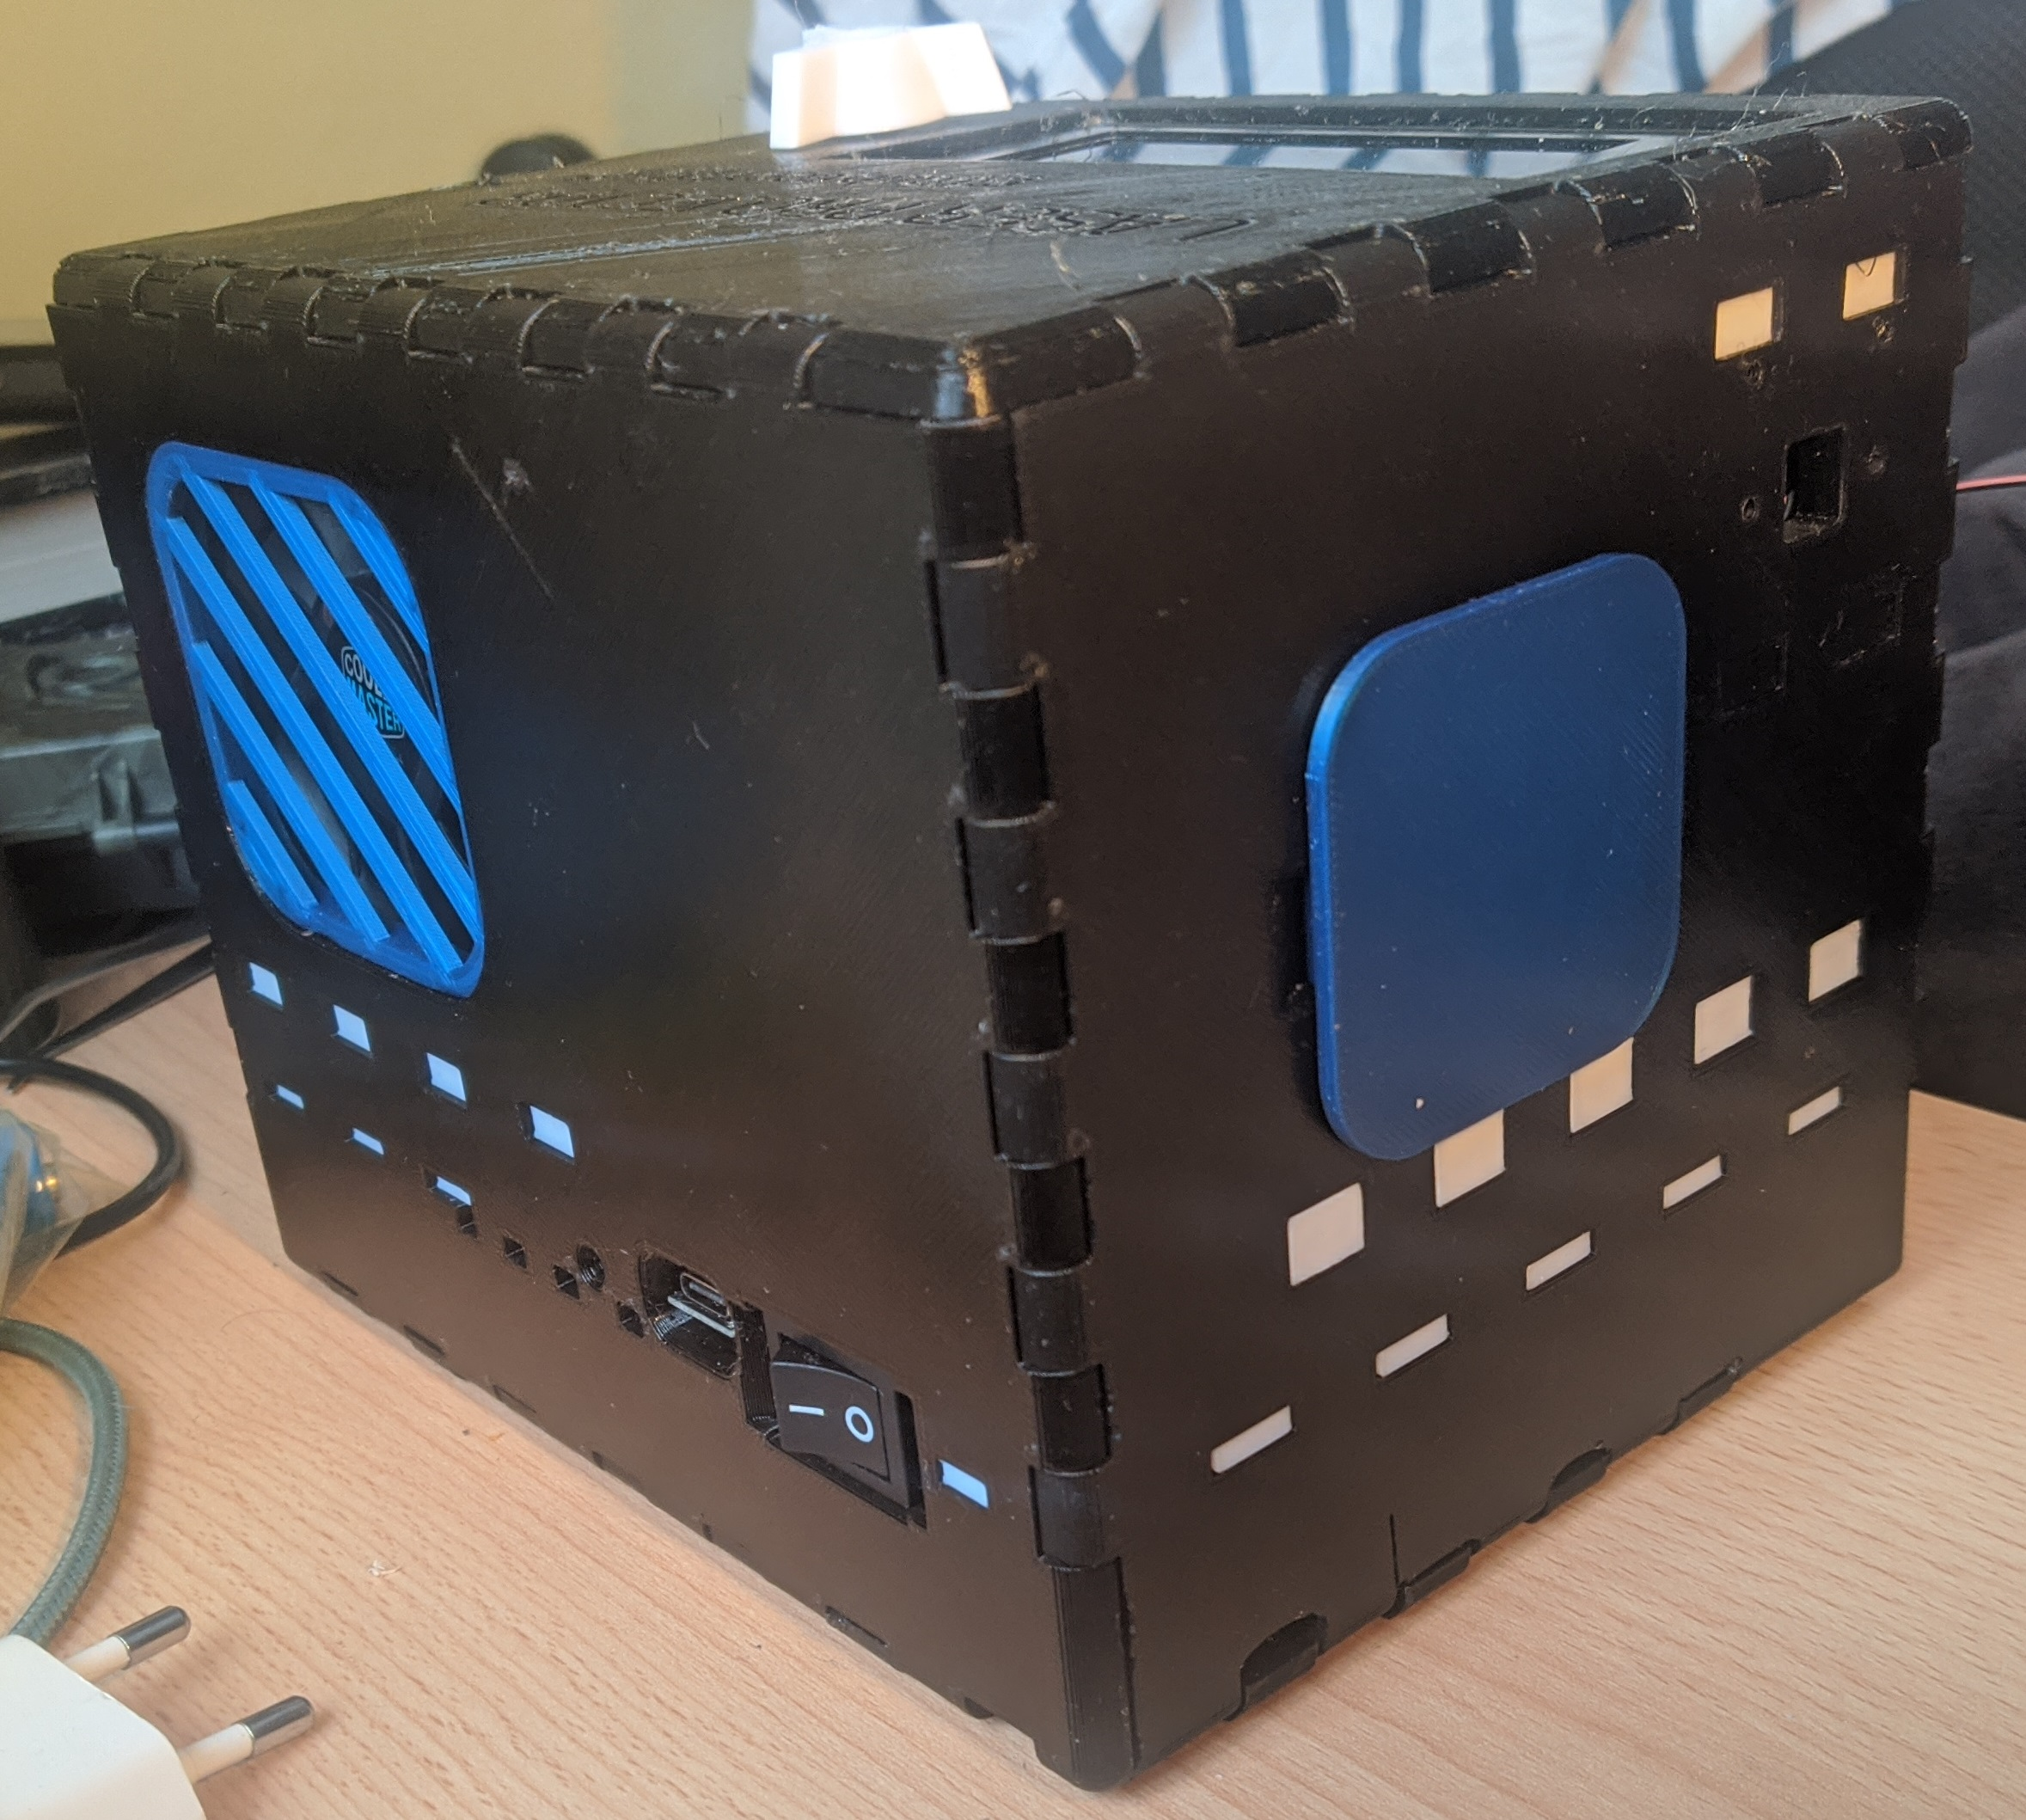
\includegraphics[width=1\textwidth]{img/hw_sides_backleft.jpg}
  \caption{\label{fig:hw_sides_backleft.jpg} Pohled na~projektor ze~strany hrany sousedící se~zadní a~pravou boční stěnou}
\end{figure}

\fxnote{fotka zepredu a~zprava}

